%! alt Clock face at 3:40 with its centre O. The minute hand points at the 8, which is 240 degrees clockwise from the 12. The hour hand points two thirds of the way from the 3 to the 4, which is 110 degrees clockwise from the 12. The smaller angle between the hands is marked 130 degrees.
%! after_paragraph 1
%! scale 3/100
% The shared preamble of every Kyuclid figure. pipeline/figures turns these colours into theme-aware paint,
% and refuses any other colour, so draw only with them:
%   figink (lines and labels), figaux (construction lines), figaccent (the object the argument turns on),
%   figtint and figaccenttint (light fills).
\documentclass[border=1.5pt]{standalone}
\usepackage{tkz-euclide}
\definecolor{figink}{RGB}{0,0,0}
\definecolor{figaux}{RGB}{85,85,85}
\definecolor{figaccent}{RGB}{192,57,43}
\definecolor{figtint}{RGB}{221,221,221}
\definecolor{figaccenttint}{RGB}{245,213,208}
% tkz-euclide's defaults draw circles, compasses and marks in 50% grey and fill points with a tint.
\makeatletter
\def\tkz@otherlinecolor{figink}
\def\tkz@euc@circlecolor{figink}
\def\tkz@euc@compasscolor{figink}
\def\tkz@euc@mkcolor{figink}
\def\tkz@mk@fill{figink}
\def\tkz@euc@pointfillcolor{figink}
\makeatother
\tkzSetUpLine[color=figink,line width=.7pt]
\tkzSetUpArc[color=figink,line width=.7pt]
\tkzSetUpCompass[color=figink,line width=.5pt]
\tkzSetUpPoint[color=figink,fill=figink,size=3.1pt]
\tikzset{
  every picture/.style={line cap=round,line join=round,color=figink},
  circle style/.append style={color=figink,line width=.7pt},
  aux/.style={color=figaux,line width=.45pt,dash pattern=on 2.6pt off 2pt},
  key/.style={color=figaccent,line width=1pt},
  mk/.style={color=figink,line width=.5pt},
  lbl/.style={color=figink,inner sep=2.2pt},
  len/.style={color=figink,inner sep=1.5pt,font=\small},
}

\begin{document}
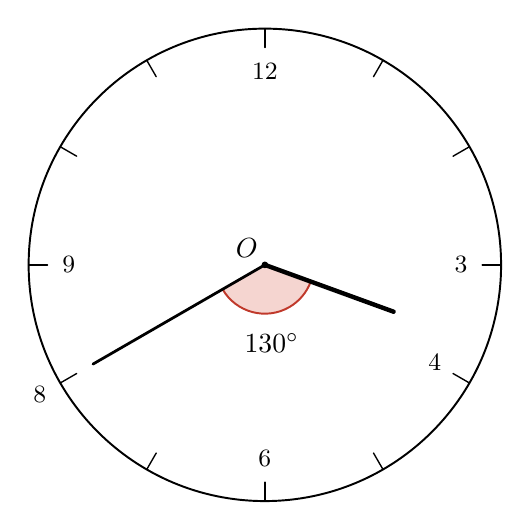
\begin{tikzpicture}
\tkzDefPoint(0.0,0.0){O} %! O = (0, 0)
\tkzDefPoint(0.0,3.0000000){R} %! R = (0, 100)
\tkzDefPoint(1.6350652,-0.59511505){H} %! H = polar(O, 58, 90 - 110)
\tkzDefPoint(-2.1823840,-1.2600000){M} %! M = polar(O, 84, 90 - 240)
\tkzDefPoint(1.3800000,2.3902301){T1} %! T1 = polar(O, 92, 60)
\tkzDefPoint(1.5000000,2.5980762){U1} %! U1 = polar(O, 100, 60)
\tkzDefPoint(2.3902301,1.3800000){T2} %! T2 = polar(O, 92, 30)
\tkzDefPoint(2.5980762,1.5000000){U2} %! U2 = polar(O, 100, 30)
\tkzDefPoint(2.7600000,0.0){T3} %! T3 = polar(O, 92, 0)
\tkzDefPoint(3.0000000,0.0){U3} %! U3 = polar(O, 100, 0)
\tkzDefPoint(2.3902301,-1.3800000){T4} %! T4 = polar(O, 92, -30)
\tkzDefPoint(2.5980762,-1.5000000){U4} %! U4 = polar(O, 100, -30)
\tkzDefPoint(1.3800000,-2.3902301){T5} %! T5 = polar(O, 92, -60)
\tkzDefPoint(1.5000000,-2.5980762){U5} %! U5 = polar(O, 100, -60)
\tkzDefPoint(0.0000000000000000000000000000000000000000000000000059820705,-2.7600000){T6} %! T6 = polar(O, 92, -90)
\tkzDefPoint(0.0000000000000000000000000000000000000000000000000065022505,-3.0000000){U6} %! U6 = polar(O, 100, -90)
\tkzDefPoint(-1.3800000,-2.3902301){T7} %! T7 = polar(O, 92, -120)
\tkzDefPoint(-1.5000000,-2.5980762){U7} %! U7 = polar(O, 100, -120)
\tkzDefPoint(-2.3902301,-1.3800000){T8} %! T8 = polar(O, 92, -150)
\tkzDefPoint(-2.5980762,-1.5000000){U8} %! U8 = polar(O, 100, -150)
\tkzDefPoint(-2.7600000,0.000000000000000000000000000000000000000000000000011964141){T9} %! T9 = polar(O, 92, 180)
\tkzDefPoint(-3.0000000,0.000000000000000000000000000000000000000000000000013004501){U9} %! U9 = polar(O, 100, 180)
\tkzDefPoint(-2.3902301,1.3800000){T10} %! T10 = polar(O, 92, 150)
\tkzDefPoint(-2.5980762,1.5000000){U10} %! U10 = polar(O, 100, 150)
\tkzDefPoint(-1.3800000,2.3902301){T11} %! T11 = polar(O, 92, 120)
\tkzDefPoint(-1.5000000,2.5980762){U11} %! U11 = polar(O, 100, 120)
\tkzDefPoint(0.0000000000000000000000000000000000000000000000000059820705,2.7600000){T12} %! T12 = polar(O, 92, 90)
\tkzDefPoint(0.0000000000000000000000000000000000000000000000000065022505,3.0000000){U12} %! U12 = polar(O, 100, 90)
\tkzDefPoint(0.0000000000000000000000000000000000000000000000000053318454,2.4600000){L12} %! L12 = polar(O, 82, 90)
\tkzDefPoint(2.4900000,0.0){L3} %! L3 = polar(O, 83, 0)
\tkzDefPoint(2.1564033,-1.2450000){L4} %! L4 = polar(O, 83, -30)
\tkzDefPoint(0.0000000000000000000000000000000000000000000000000053318454,-2.4600000){L6} %! L6 = polar(O, 82, -90)
\tkzDefPoint(-2.4900000,0.000000000000000000000000000000000000000000000000010793736){L9} %! L9 = polar(O, 83, 180)
\tkzDefPoint(-2.8578838,-1.6500000){L8} %! L8 = polar(O, 110, -150)
%! fact angle(H, O, M) == 130
%! fact angle(U12, O, H) == 110
%! fact angle(U12, O, M) == 360 - 240
%! fact collinear(M, O, U8)
%! fact on_circle(R, O, 100)
\tkzFillAngle[size=.62,color=figaccenttint](M,O,H)
\tkzDrawCircle(O,R)
\tkzDrawSegments[mk](T1,U1 T2,U2 T3,U3 T4,U4 T5,U5 T6,U6 T7,U7 T8,U8 T9,U9 T10,U10 T11,U11 T12,U12)
\tkzMarkAngle[size=.62,arc=l,mark=none,color=figaccent,line width=.7pt](M,O,H)
\tkzDrawSegment[line width=1.6pt](O,H)
\tkzDrawSegment[line width=1pt](O,M)
\tkzDrawPoint(O)
\tkzLabelPoint[above left,lbl](O){$O$}
\tkzLabelAngle[pos=1.0](M,O,H){$130^\circ$}
\tkzLabelPoint[anchor=center,len](L12){$12$}
\tkzLabelPoint[anchor=center,len](L3){$3$}
\tkzLabelPoint[anchor=center,len](L6){$6$}
\tkzLabelPoint[anchor=center,len](L9){$9$}
\tkzLabelPoint[anchor=center,len](L4){$4$}
\tkzLabelPoint[anchor=center,len](L8){$8$}
\end{tikzpicture}
\end{document}
